\documentclass[12pt,draft]{report}
\usepackage{graphicx} % Required for inserting images
\usepackage{multirow}
\usepackage{lscape}
\usepackage{pdflscape}
\usepackage{fixltx2e}
\usepackage{geometry}
\usepackage{wasysym}
\usepackage{amsmath}
\usepackage{amssymb}
\usepackage{caption}
\usepackage{subcaption}


\newcommand{\head}[1]{\textnormal{\textbf{#1}}}
\newcommand\ion[2]{\text{#1\,\textsc{\lowercase{#2}}}}

\title{Thesis Phase-1}
\author{Sameer Patidar}
\date{July 2023}

\begin{document}


\begin{landscape}

\begin{figure}
\centering
\vspace{-20mm}
\hspace*{-35mm}
\captionsetup{oneside,margin={0cm,35mm}}
\includegraphics[width=1.25\linewidth]{System-Plots/3C263_z=0.140756_sys_plot.png}
\end{figure}

\end{landscape}


\begin{center}
 
\begin{tabular}{cccc}
        \hline \hline \tabularnewline
       \head{Ion} & \head{v (km s\textsuperscript{$\mathbf{-1}$})} & \head{b (km s\textsuperscript{$\mathbf{-1}$})} & \head{log [N cm\textsuperscript{$\mathbf{-2}$}]} 
       \tabularnewline \tabularnewline \hline \tabularnewline 

\ion{Si}{iii}  &    -18 $\pm$ 8   &    35 $\pm$ 11    &     12.39 $\pm$ 0.09 \\
\ion{C}{iv}   &    -10 $\pm$ 3   &    33 $\pm$ 0    &     13.71 $\pm$ 0.04 \\
\ion{O}{vi}   &    0 $\pm$ 2   &    26 $\pm$ 4    &     13.63 $\pm$ 0.04 \\
\ion{H}{i}   &    -14 $\pm$ 1   &    87 $\pm$ 10    &     13.49 $\pm$ 0.06 \\
\ion{H}{i}   &    0 $\pm$ 1   &    28 $\pm$ 1    &     14.49 $\pm$ 0.02 \\
\tabularnewline \hline \hline \tabularnewline

\end{tabular}

\end{center}

N(\ion{H}{I})=13.49 \\

Excluding \ion{O}{vi} : $n_H$ = -3.88 $\pm$ 0.04 \hspace{10mm} $Z$ = 1.06 $\pm$ 0.05

Including \ion{O}{vi} : $n_H$ = -4.13 $\pm$ 0.02 \hspace{10mm} $Z$ = 0.99 $\pm$ 0.04
\\\\
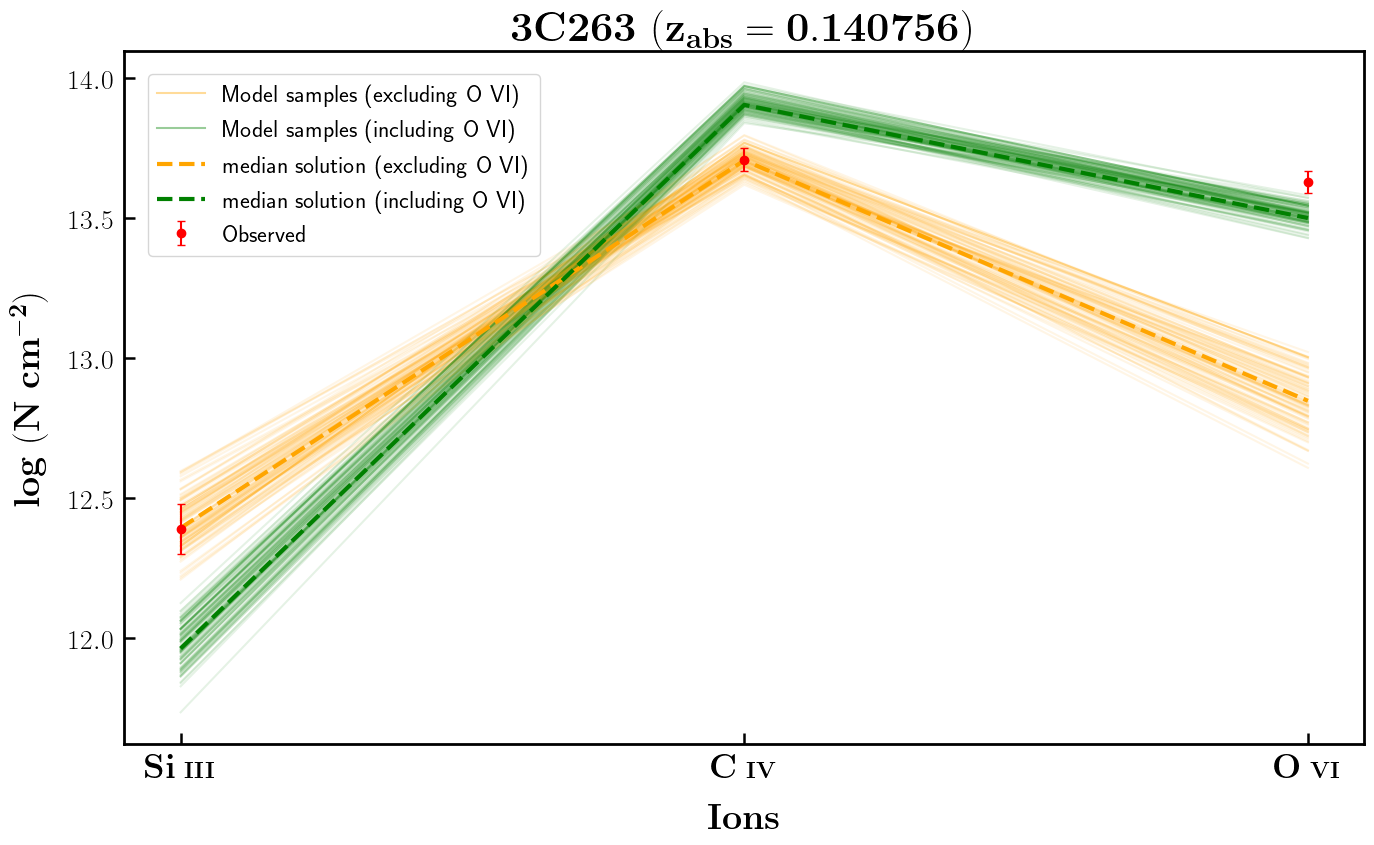
\includegraphics[width=1\linewidth]{Ionisation-Modelling-Plots/3c263-z=0.140756-compI.png}


\newpage


\begin{landscape}

    \begin{figure}
    \centering
    \vspace{-20mm}
    \hspace*{-35mm}
    \captionsetup{oneside,margin={0cm,35mm}}
    \includegraphics[width=1.25\linewidth]{System-Plots/PKS0637-752_z=0.161064_sys_plot.png}
    \end{figure}
    
\end{landscape}


\begin{center}
 
    \begin{tabular}{cccc}
            \hline \hline \tabularnewline
           \head{Ion} & \head{v (km s\textsuperscript{$\mathbf{-1}$})} & \head{b (km s\textsuperscript{$\mathbf{-1}$})} & \head{log [N cm\textsuperscript{$\mathbf{-2}$}]} 
           \tabularnewline \tabularnewline \hline \tabularnewline 
    
           \ion{N}{v}   &    -42.0 $\pm$ 6.0   &    40 $\pm$ 9    &     13.37 $\pm$ 0.07 \\
           \ion{Si}{iii}   &    11.0 $\pm$ 4.0   &    30 $\pm$ 7    &     12.37 $\pm$ 0.06 \\
           \ion{O}{vi}   &    0.0 $\pm$ 3.0   &    48 $\pm$ 5    &     14.02 $\pm$ 0.03 \\
           \ion{H}{i}   &    -13.0 $\pm$ 2.0   &    162 $\pm$ 21    &     13.6 $\pm$ 0.06 \\
           \ion{H}{i}   &    -1.0 $\pm$ 1.0   &    45 $\pm$ 1    &     15.01 $\pm$ 0.02 \\
    \tabularnewline \hline \hline \tabularnewline
    
    \end{tabular}
    
    \end{center}
    
    N(\ion{H}{I})=13.60 \\
    
    Excluding \ion{O}{vi} : $n_H$ = -4.05 $\pm$ 0.03 \hspace{10mm} $Z$ = 1.20 $\pm$ 0.05
    
    Including \ion{O}{vi} : $n_H$ = -4.12 $\pm$ 0.01 \hspace{10mm} $Z$ = 1.30 $\pm$ 0.04
    \\\\
    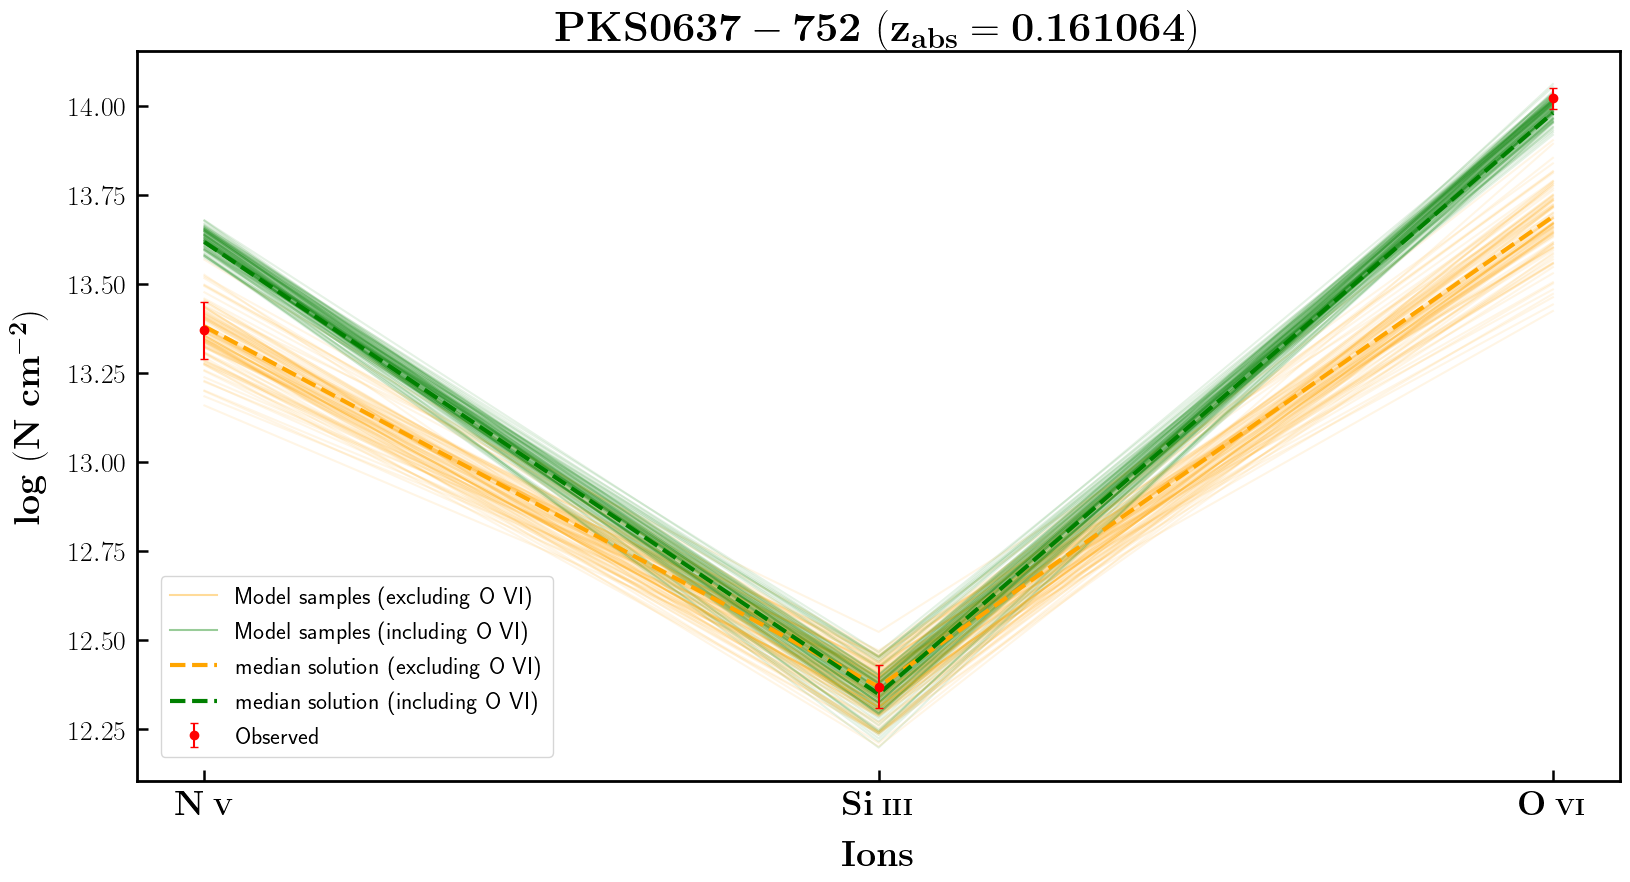
\includegraphics[width=1\linewidth]{Ionisation-Modelling-Plots/pks0637-z=0.161064-compI.png}



\newpage


\begin{landscape}

    \begin{figure}
    \centering
    \vspace{-20mm}
    \hspace*{-35mm}
    \captionsetup{oneside,margin={0cm,35mm}}
    \includegraphics[width=1.25\linewidth]{System-Plots/PKS0637-752_z=0.417539_sys_plot.png}
    \end{figure}
    
\end{landscape}


\begin{center}
    
    \begin{tabular}{cccc}
        \hline \hline \tabularnewline
        \head{Ion} & \head{v (km s\textsuperscript{$\mathbf{-1}$})} & \head{b (km s\textsuperscript{$\mathbf{-1}$})} & \head{log [N cm\textsuperscript{$\mathbf{-2}$}]} 
        \tabularnewline \tabularnewline \hline \tabularnewline 
    
        \ion{Si}{iii}   &    -5.0 $\pm$ 4.0   &    35 $\pm$ 7    &     12.74 $\pm$ 0.06 \\
        \ion{C}{iii}   &    -4.0 $\pm$ 1.0   &    24 $\pm$ 2    &     14.44 $\pm$ 0.15 \\
        \ion{O}{vi}   &    0.0 $\pm$ 1.0   &    42 $\pm$ 6    &     14.19 $\pm$ 0.05 \\
        \ion{H}{i}   &    -17.0 $\pm$ 1.0   &    30 $\pm$ 1    &     15.41 $\pm$ 0.03 \\
        \ion{H}{i}   &    20.0 $\pm$ 1.0   &    46 $\pm$ 4    &     14.61 $\pm$ 0.07 \\
        
        \tabularnewline \hline \hline \tabularnewline
    
    \end{tabular}
    
\end{center}
    
N(\ion{H}{I})=15.41 \\

Excluding \ion{O}{vi} : $n_H$ = -3.54 $\pm$ 0.11 \hspace{10mm} $Z$ = -0.49 $\pm$ 0.11

Including \ion{O}{vi} : $n_H$ = -3.74 $\pm$ 0.02 \hspace{10mm} $Z$ = -0.23 $\pm$ 0.04 \\

NOTE : MCMC walkers initialised near the solution for excluding \ion{O}{vi} case.
\\\\
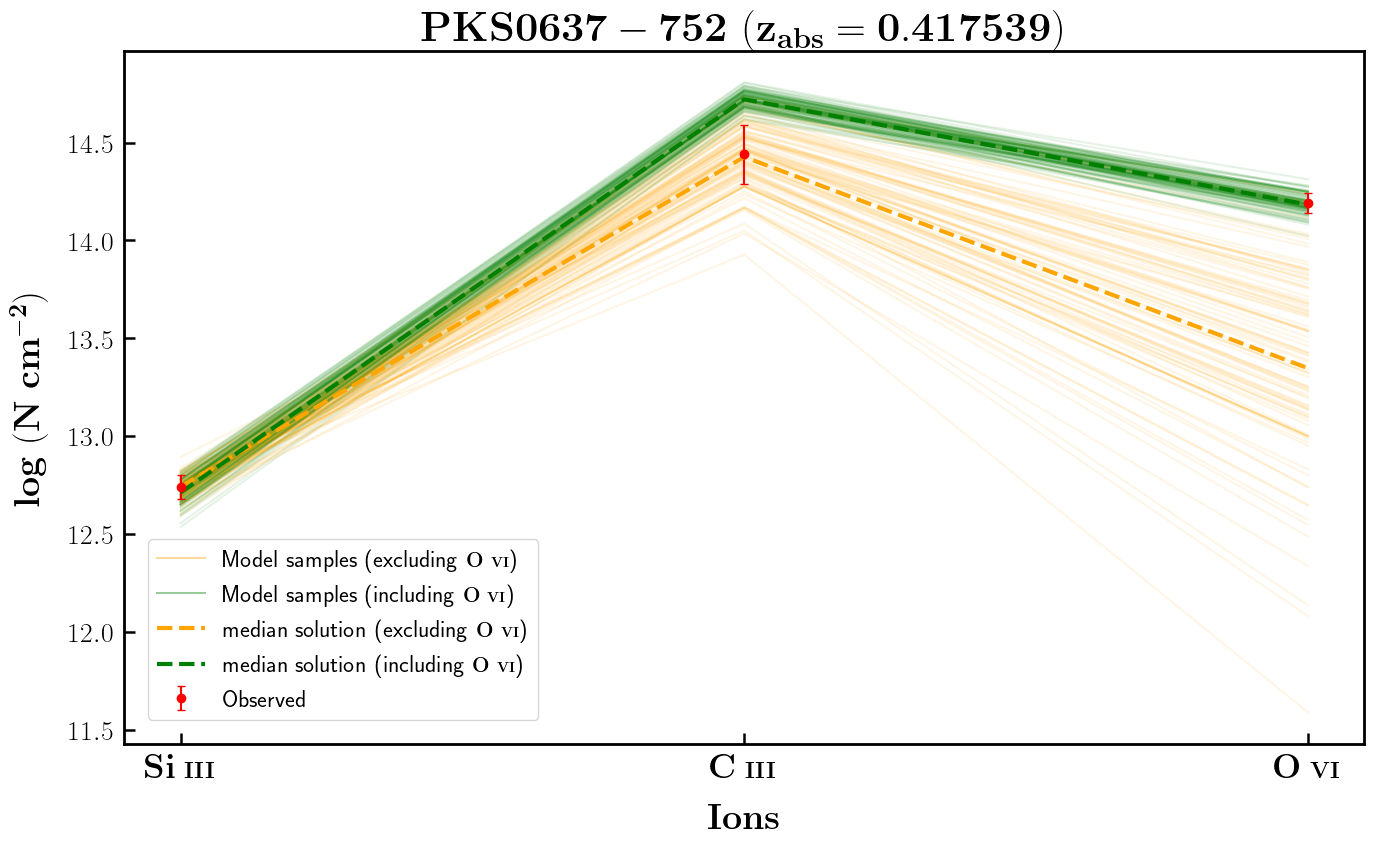
\includegraphics[width=1\linewidth]{Ionisation-Modelling-Plots/pks0637-z=0.417539-compI.png}




\newpage


\begin{landscape}

    \begin{figure}
    \centering
    \vspace{-20mm}
    \hspace*{-35mm}
    \captionsetup{oneside,margin={0cm,35mm}}
    \includegraphics[width=1.25\linewidth]{System-Plots/PG1424+240_z=0.147104_sys_plot.png}
    \end{figure}
    
\end{landscape}


\begin{center}
    
    \begin{tabular}{cccc}
            \hline \hline \tabularnewline
            \head{Ion} & \head{v (km s\textsuperscript{$\mathbf{-1}$})} & \head{b (km s\textsuperscript{$\mathbf{-1}$})} & \head{log [N cm\textsuperscript{$\mathbf{-2}$}]} 
            \tabularnewline \tabularnewline \hline \tabularnewline 
    
            \ion{C}{iv}   &    -81.0 $\pm$ 2.0   &    11 $\pm$ 4    &     13.58 $\pm$ 0.09 \\
            \ion{C}{iv}   &    -18.0 $\pm$ 2.0   &    20 $\pm$ 3    &     14.06 $\pm$ 0.05 \\ \tabularnewline
            \ion{Si}{iii}   &    -78.0 $\pm$ 2.0   &    15 $\pm$ 3    &     12.58 $\pm$ 0.05 \\
            \ion{Si}{iii}   &    -9.0 $\pm$ 1.0   &    16 $\pm$ 2    &     12.87 $\pm$ 0.03 \\ \tabularnewline
            \ion{Si}{iv}   &    -82.0 $\pm$ 4.0   &    13 $\pm$ 7    &     12.69 $\pm$ 0.1 \\
            \ion{Si}{iv}   &    -11.0 $\pm$ 2.0   &    11 $\pm$ 5    &     12.88 $\pm$ 0.07 \\ \tabularnewline
            \ion{O}{vi}   &    -56.0 $\pm$ 9.0   &    39 $\pm$ 13    &     13.77 $\pm$ 0.11 \\
            \ion{O}{vi}   &    4.0 $\pm$ 4.0   &    16 $\pm$ 6    &     13.73 $\pm$ 0.11 \\ \tabularnewline
            \ion{H}{i}   &    -454.0 $\pm$ 3.0   &    27 $\pm$ 5    &     13.16 $\pm$ 0.05 \\
            \ion{H}{i}   &    -87.0 $\pm$ 3.0   &    23 $\pm$ 2    &     14.88 $\pm$ 0.05 \\
            \ion{H}{i}   &    0.0 $\pm$ 3.0   &    29 $\pm$ 2    &     15.44 $\pm$ 0.14 \\
            \ion{H}{i}   &    216.0 $\pm$ 2.0   &    40 $\pm$ 3    &     13.49 $\pm$ 0.02 \\
            \tabularnewline \hline \hline \tabularnewline
    
    \end{tabular}
    
    \end{center}
    
    N(\ion{H}{I})=15.44 \\
    
    Excluding \ion{O}{vi} : $n_H$ = -3.81 $\pm$ 0.03 \hspace{10mm} $Z$ = -0.46 $\pm$ 0.03
    
    Including \ion{O}{vi} : $n_H$ = -3.88 $\pm$ 0.02 \hspace{10mm} $Z$ = -0.42 $\pm$ 0.02
    \\\\

    N(\ion{H}{I})=14.88 \\
    
    Excluding \ion{O}{vi} : $n_H$ = -3.74 $\pm$ 0.05 \hspace{10mm} $Z$ = -0.22 $\pm$ 0.04
    
    Including \ion{O}{vi} : $n_H$ = -3.96 $\pm$ 0.03 \hspace{10mm} $Z$ = -0.07 $\pm$ 0.04
    \\\\

    \newpage

    \begin{figure}[!h]
        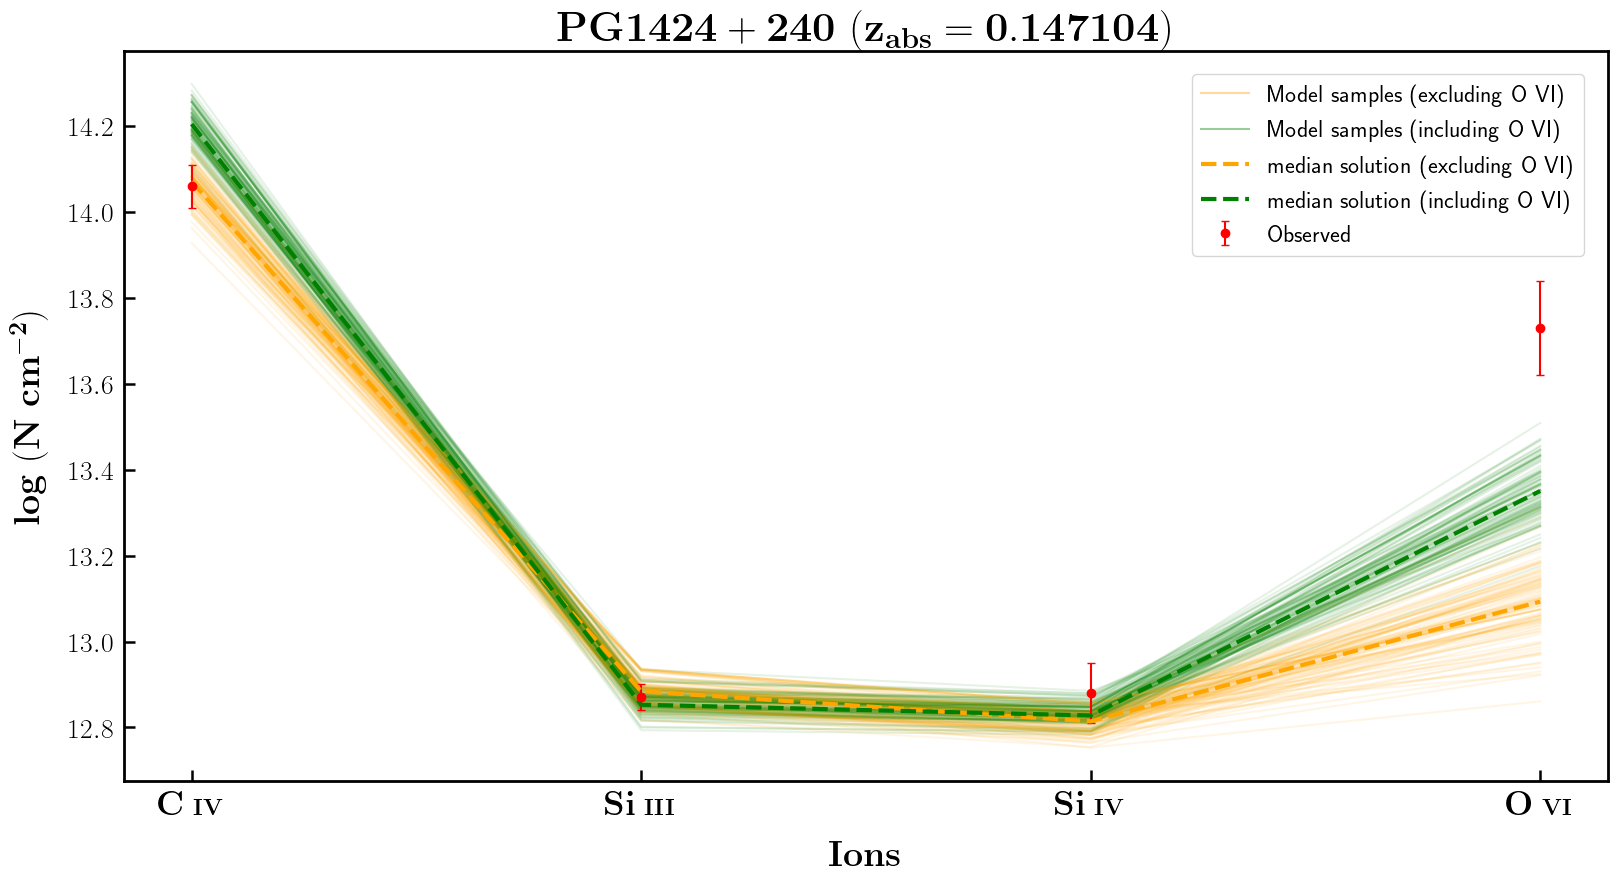
\includegraphics[width=0.9\linewidth]{Ionisation-Modelling-Plots/pg1424-z=0.147104-compIII.png}
        \caption{N(\ion{H}{i})=15.44}
    \end{figure}

    \begin{figure}[!b]
        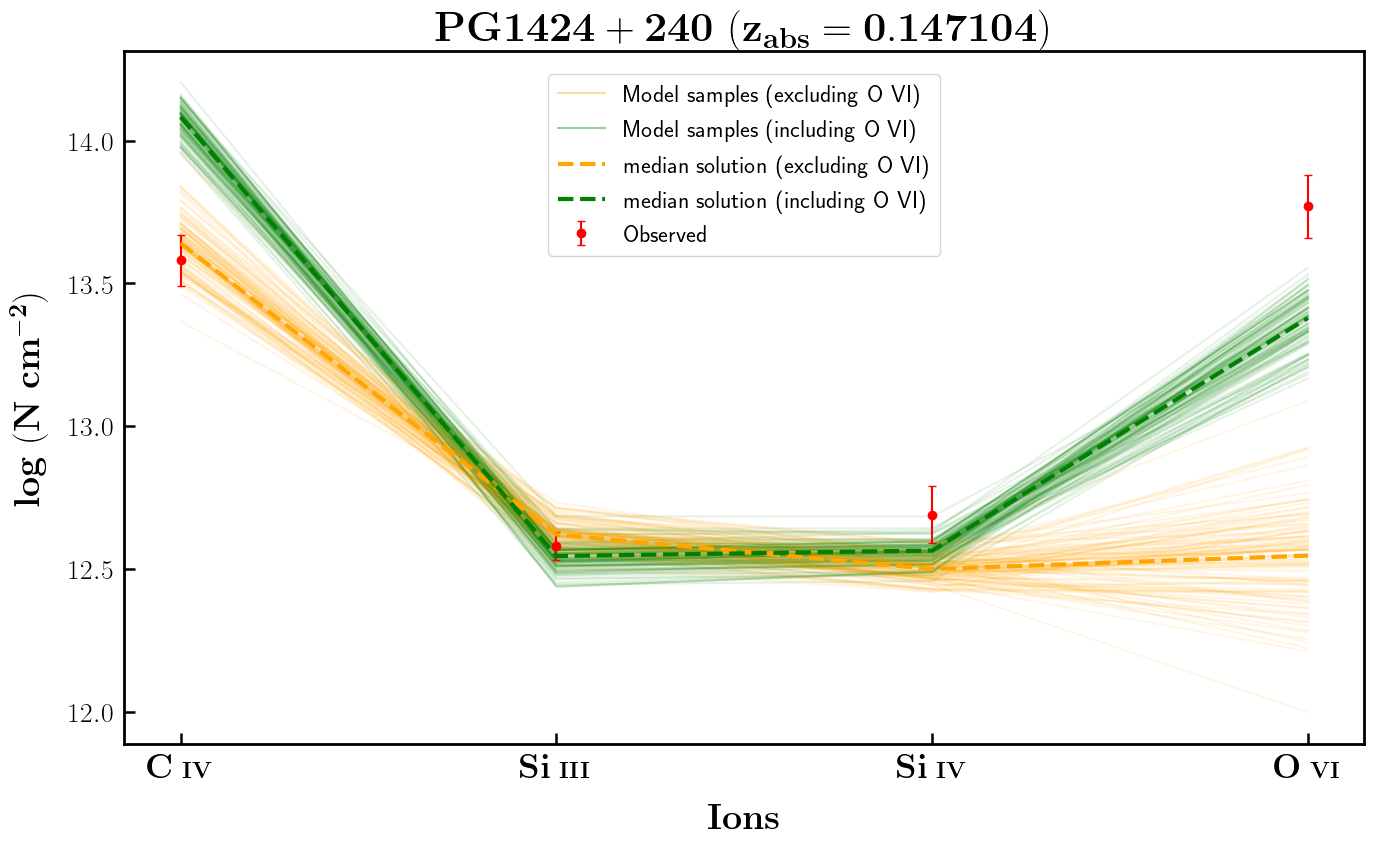
\includegraphics[width=0.9\linewidth]{Ionisation-Modelling-Plots/pg1424-z=0.147104-compII.png}
        \caption{N(\ion{H}{i})=14.88}
    \end{figure}

\newpage


\begin{landscape}

    \begin{figure}
    \centering
    \vspace{-20mm}
    \hspace*{-35mm}
    \captionsetup{oneside,margin={0cm,35mm}}
    \includegraphics[width=1.25\linewidth]{System-Plots/PG0003+158_z=0.386089_sys_plot.png}
    \end{figure}
    
\end{landscape}


\begin{center}
    
    \begin{tabular}{cccc}
        \hline \hline \tabularnewline
        \head{Ion} & \head{v (km s\textsuperscript{$\mathbf{-1}$})} & \head{b (km s\textsuperscript{$\mathbf{-1}$})} & \head{log [N cm\textsuperscript{$\mathbf{-2}$}]} 
        \tabularnewline \tabularnewline \hline \tabularnewline 
    
        \ion{O}{iii}   &    -18.0 $\pm$ 2.0   &    9 $\pm$ 5    &     13.93 $\pm$ 0.08 \\
        \ion{C}{iii}   &    -11.0 $\pm$ 1.0   &    13 $\pm$ 2    &     13.35 $\pm$ 0.05 \\
        \ion{N}{v}   &    -7.0 $\pm$ 1.0   &    33 $\pm$ 11    &     13.49 $\pm$ 0.11 \\
        \ion{O}{vi}   &    0.0 $\pm$ 2.0   &    25 $\pm$ 3    &     13.87 $\pm$ 0.04 \\
        \ion{O}{vi}   &    54.0 $\pm$ 3.0   &    25 $\pm$ 4    &     13.71 $\pm$ 0.06 \\
        \ion{H}{i}   &    -10.0 $\pm$ 1.0   &    29 $\pm$ 0    &     14.81 $\pm$ 0.03 \\
        \ion{H}{i}   &    40.0 $\pm$ 9.0   &    40 $\pm$ 4    &     14.1 $\pm$ 0.05 \\

        \tabularnewline \hline \hline \tabularnewline
    
    \end{tabular}
    
\end{center}
    
N(\ion{H}{I})=14.81 \\

Excluding \ion{O}{vi} : $n_H$ = -4.12 $\pm$ 0.06 \hspace{10mm} $Z$ = -0.65 $\pm$ 0.04

Including \ion{O}{vi} : $n_H$ = -4.07 $\pm$ 0.02 \hspace{10mm} $Z$ = -0.68 $\pm$ 0.03
\\\\
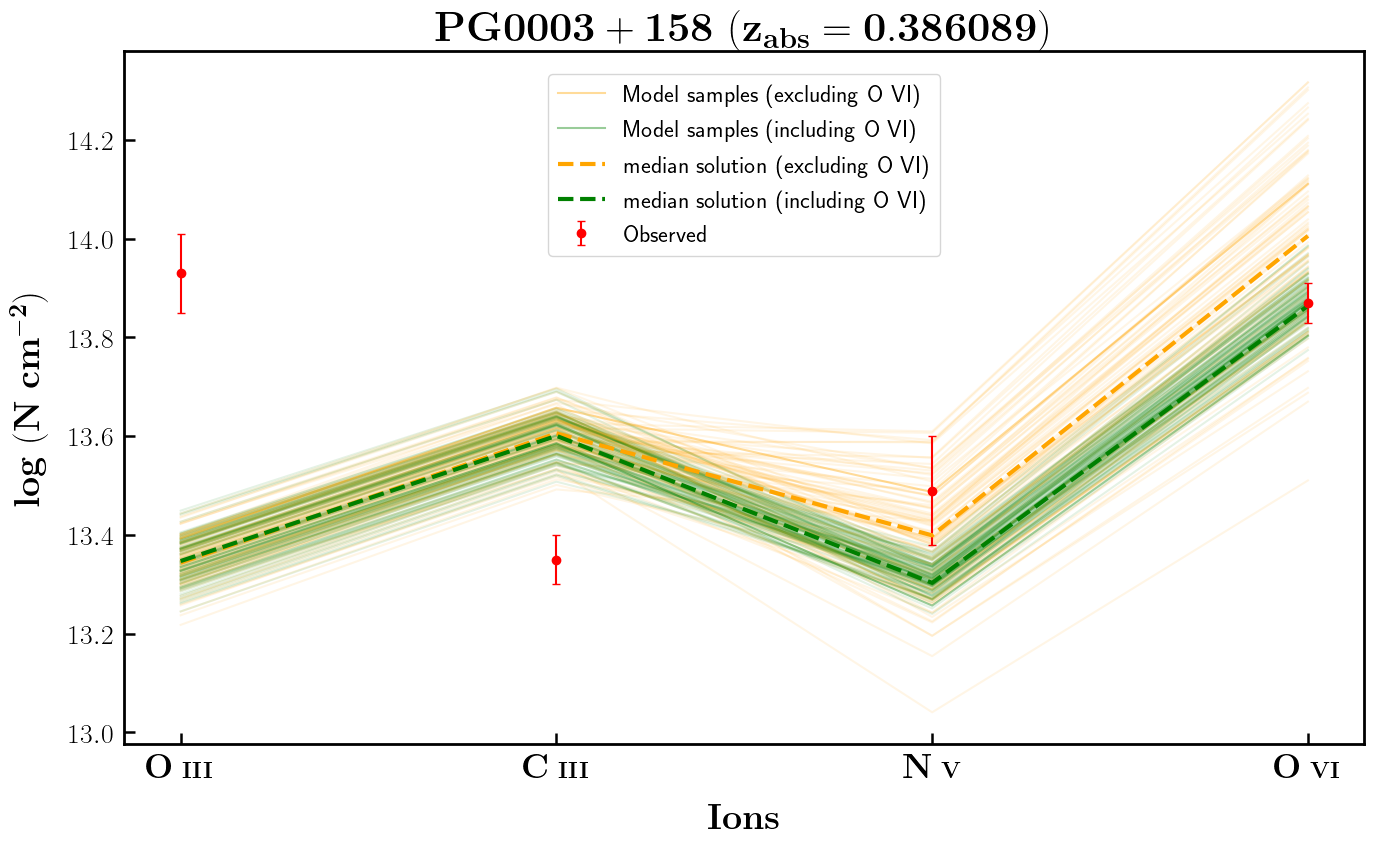
\includegraphics[width=1\linewidth]{Ionisation-Modelling-Plots/pg0003-z=0.386089-compI.png}



\newpage


\begin{landscape}

    \begin{figure}
    \centering
    \vspace{-20mm}
    \hspace*{-35mm}
    \captionsetup{oneside,margin={0cm,35mm}}
    \includegraphics[width=1.25\linewidth]{System-Plots/PG0003+158_z=0.421923_sys_plot.png}
    \end{figure}
    
\end{landscape}


\begin{center}
    
    \begin{tabular}{cccc}
        \hline \hline \tabularnewline
        \head{Ion} & \head{v (km s\textsuperscript{$\mathbf{-1}$})} & \head{b (km s\textsuperscript{$\mathbf{-1}$})} & \head{log [N cm\textsuperscript{$\mathbf{-2}$}]} 
        \tabularnewline \tabularnewline \hline \tabularnewline 
    
        \ion{C}{iii}   &    -9.0 $\pm$ 1.0   &    13 $\pm$ 1    &     13.35 $\pm$ 0.04 \\
        \ion{O}{iii}   &    -1.0 $\pm$ 2.0   &    7 $\pm$ 5    &     13.83 $\pm$ 0.13 \\
        \ion{O}{vi}   &    0.0 $\pm$ 1.0   &    27 $\pm$ 1    &     14.27 $\pm$ 0.02 \\
        \ion{H}{i}   &    -272.0 $\pm$ 6.0   &    66 $\pm$ 10    &     13.37 $\pm$ 0.05 \\
        \ion{H}{i}   &    -16.0 $\pm$ 1.0   &    64 $\pm$ 3    &     14.17 $\pm$ 0.04 \\
        \ion{H}{i}   &    -2.0 $\pm$ 1.0   &    26 $\pm$ 1    &     14.71 $\pm$ 0.02 \\
    
        \tabularnewline \hline \hline \tabularnewline
    
    \end{tabular}
    
\end{center}
    
N(\ion{H}{I})=14.17 \\

Excluding \ion{O}{vi} : $n_H$ = -2.66 $\pm$ 0.22 \hspace{10mm} $Z$ = 0.42 $\pm$ 0.23

Including \ion{O}{vi} : $n_H$ = -4.24 $\pm$ 0.02 \hspace{10mm} $Z$ = -0.09 $\pm$ 0.03 \\

NOTE : Convergence is not good for excluding \ion{O}{vi} case
\\\\
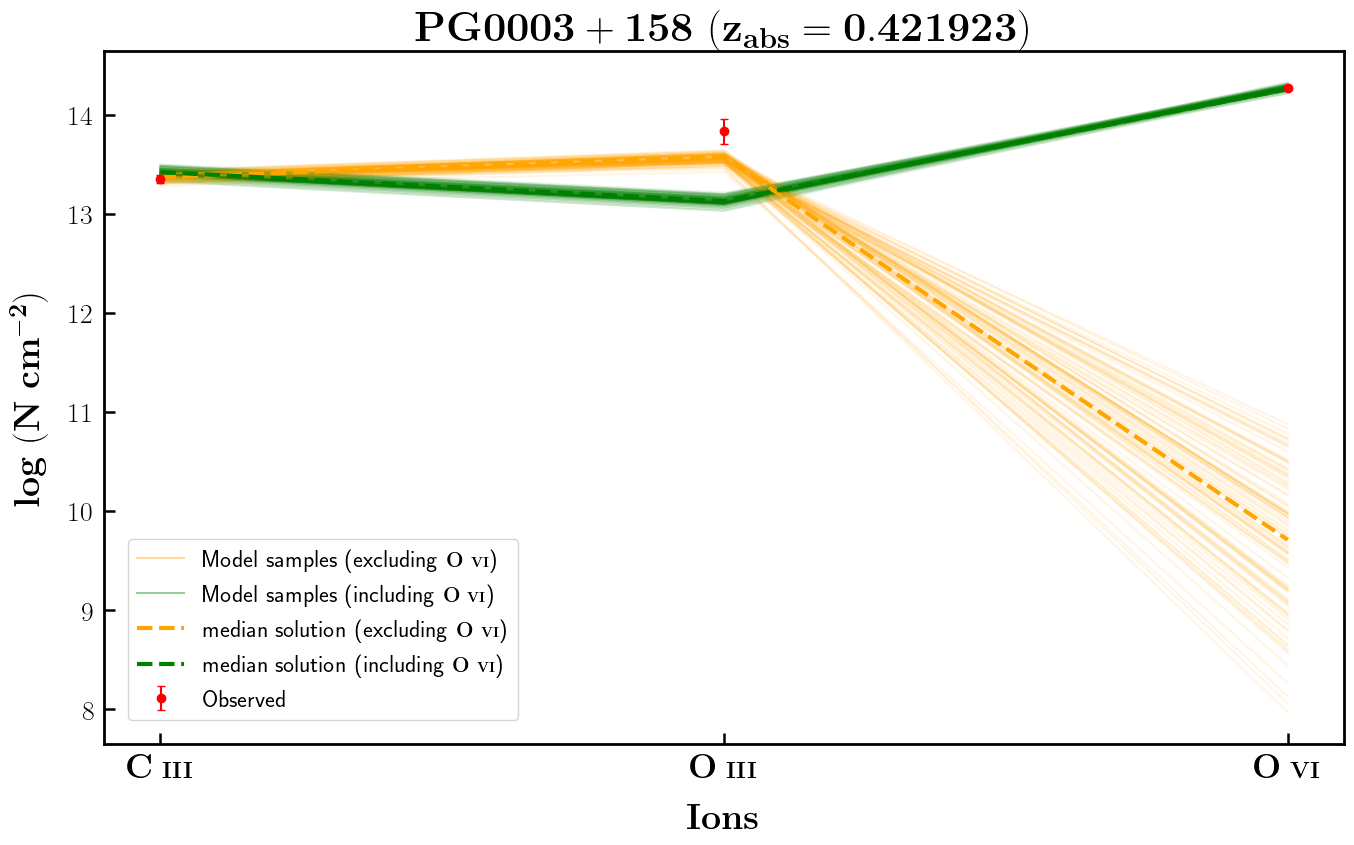
\includegraphics[width=1\linewidth]{Ionisation-Modelling-Plots/pg0003-z=0.421923-compII.png}
    


\newpage


\begin{landscape}

    \begin{figure}
    \centering
    \vspace{-20mm}
    \hspace*{-35mm}
    \captionsetup{oneside,margin={0cm,35mm}}
    \includegraphics[width=1.25\linewidth]{System-Plots/PG1216+069_z=0.282286_sys_plot.png}
    \end{figure}
    
\end{landscape}


\begin{center}
 
\begin{tabular}{cccc}
        \hline \hline \tabularnewline
        \head{Ion} & \head{v (km s\textsuperscript{$\mathbf{-1}$})} & \head{b (km s\textsuperscript{$\mathbf{-1}$})} & \head{log [N cm\textsuperscript{$\mathbf{-2}$}]} 
        \tabularnewline \tabularnewline \hline \tabularnewline 

        \ion{Si}{iii}   &    0.0 $\pm$ 1.0   &    14 $\pm$ 3    &     12.92 $\pm$ 0.05 \\
        \ion{C}{iii}   &    -51.0 $\pm$ 3.0   &    32 $\pm$ 5    &     13.33 $\pm$ 0.05 \\
        \ion{C}{iii}   &    5.0 $\pm$ 1.0   &    16 $\pm$ 2    &     13.76 $\pm$ 0.07 \\
        \ion{O}{vi}   &    -64.0 $\pm$ 6.0   &    58 $\pm$ 9    &     13.93 $\pm$ 0.05 \\
        \ion{O}{vi}   &    19.0 $\pm$ 2.0   &    12 $\pm$ 5    &     13.54 $\pm$ 0.09 \\
        \ion{H}{i}   &    -31.0 $\pm$ 1.0   &    52 $\pm$ 3    &     15.1 $\pm$ 0.05 \\
        \ion{H}{i}   &    7.0 $\pm$ 1.0   &    22 $\pm$ 1    &     16.4 $\pm$ 0.03 \\
        \ion{H}{i}   &    169.0 $\pm$ 22.0   &    53 $\pm$ 10    &     13.15 $\pm$ 0.18 \\

        \tabularnewline \hline \hline \tabularnewline

\end{tabular}
    
\end{center}
    
N(\ion{H}{I})=15.10 \\

Excluding \ion{O}{vi} : $n_H$ = -2.13 $\pm$ 0.15 \hspace{10mm} $Z$ = 0.65 $\pm$ 0.22

Including \ion{O}{vi} : $n_H$ = -3.86 $\pm$ 0.02 \hspace{10mm} $Z$ = -0.37 $\pm$ 0.03 \\

NOTE : Convergence is not much good for excluding \ion{O}{vi} case
\\\\

N(\ion{H}{I})=16.40 \\

Excluding \ion{O}{vi} : $n_H$ = -2.08 $\pm$ 0.43 \hspace{10mm} $Z$ = -0.37 $\pm$ 0.59

Including \ion{O}{vi} : $n_H$ = -3.68 $\pm$ 0.02 \hspace{10mm} $Z$ = -1.55 $\pm$ 0.04 \\

NOTE : Convergence is not much good for excluding \ion{O}{vi} case


\newpage


\begin{figure}[!h]
    \centering
    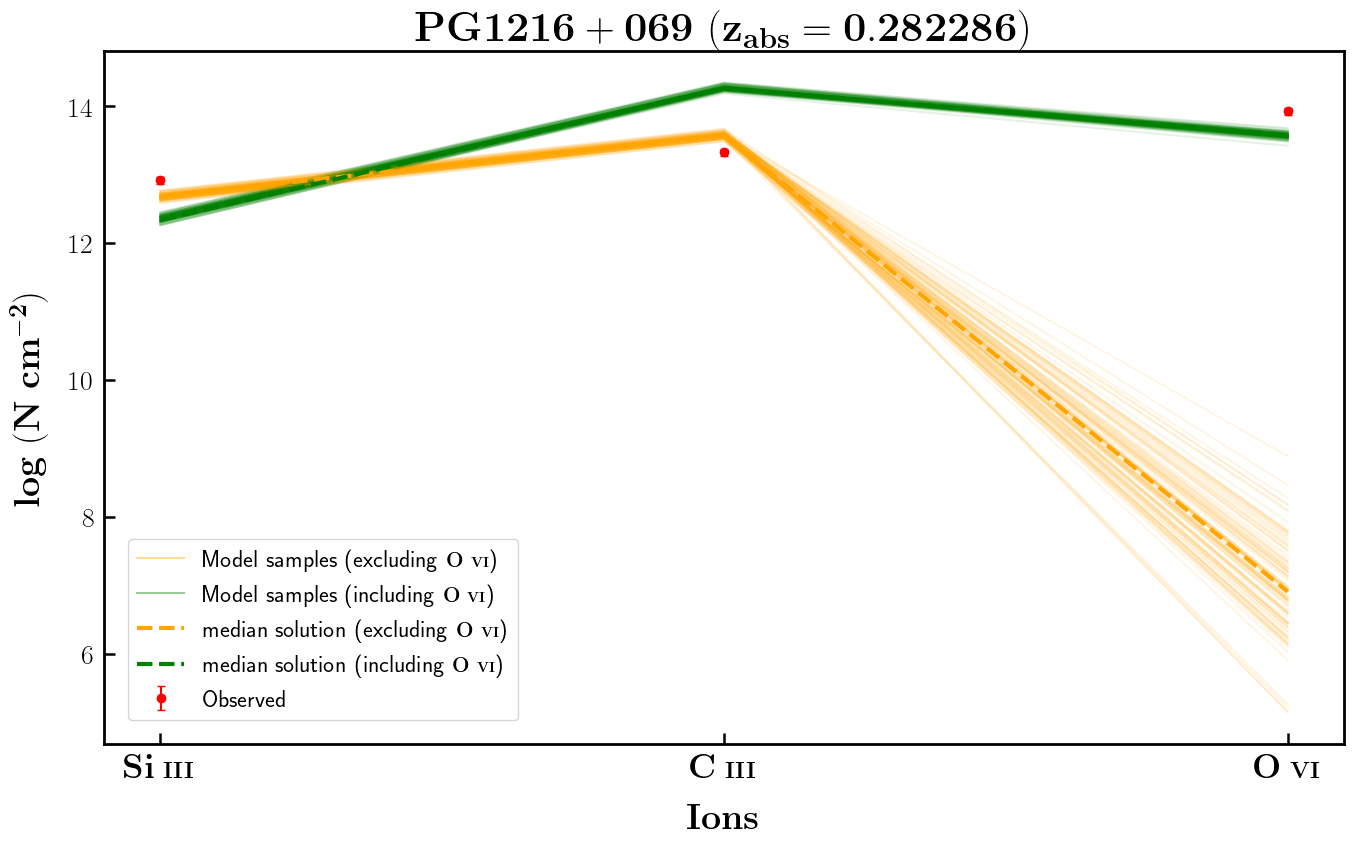
\includegraphics[width=0.85\linewidth]{Ionisation-Modelling-Plots/pg1216-z=0.282286-compI.png}
    \caption{N(\ion{H}{i})=15.10}
\end{figure}

\begin{figure}[!b]
    \centering
    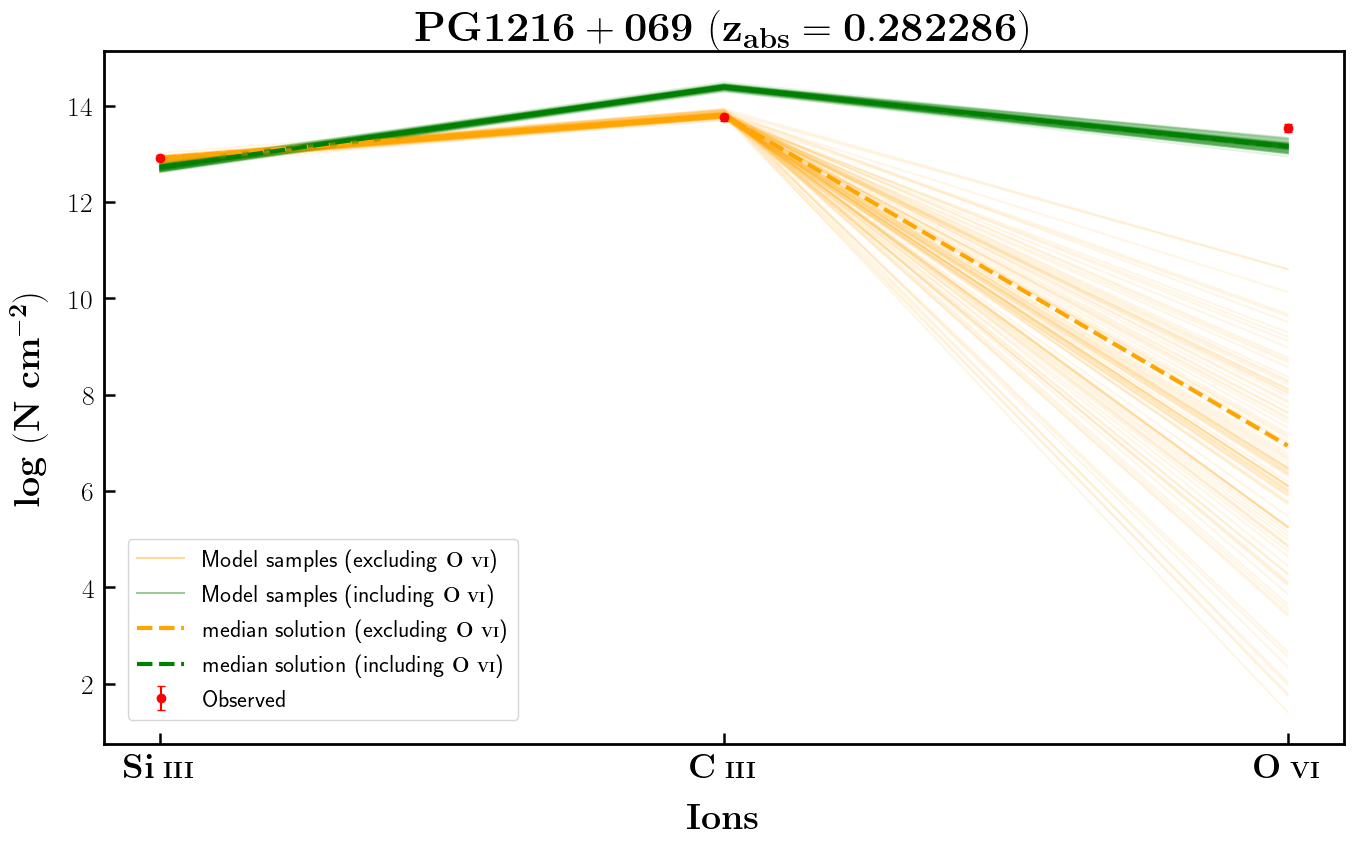
\includegraphics[width=0.85\linewidth]{Ionisation-Modelling-Plots/pg1216-z=0.282286-compII.png}
    \caption{N(\ion{H}{i})=16.40}
\end{figure}


\newpage

\begin{landscape}

\begin{figure}
    \centering
    \vspace{-20mm}
    \hspace*{-35mm}
    \captionsetup{oneside,margin={0cm,35mm}}
    \includegraphics[width=1.25\linewidth]{System-Plots/SDSSJ135712.61+170444_z=0.097869_sys_plot.png}
\end{figure}

\end{landscape}


\begin{center} 

\begin{tabular}{cccc} 

    \hline \hline \tabularnewline 
    \head{Ion} & \head{v (km s\textsuperscript{$\mathbf{-1}$})} & \head{b (km s\textsuperscript{$\mathbf{-1}$})} & \head{log [N cm\textsuperscript{$\mathbf{-2}$}]}
    \tabularnewline \tabularnewline \hline \tabularnewline 
 
    \ion{Si}{iii}   &    -62.0 $\pm$ 2.0   &    17 $\pm$ 3    &     12.94 $\pm$ 0.05 \\
    \ion{Si}{iii}   &    4.0 $\pm$ 1.0   &    13 $\pm$ 10    &     14.67 $\pm$ 2.87 \\
    \ion{C}{iv}   &    -74.0 $\pm$ 6.0   &    33 $\pm$ 1    &     13.82 $\pm$ 0.09 \\
    \ion{C}{iv}   &    -7.0 $\pm$ 8.0   &    32 $\pm$ 12    &     13.63 $\pm$ 0.12 \\
    \ion{Si}{iv}   &    -66.0 $\pm$ 4.0   &    18 $\pm$ 6    &     13.02 $\pm$ 0.08 \\
    \ion{Si}{iv}   &    0.0 $\pm$ 4.0   &    29 $\pm$ 5    &     13.3 $\pm$ 0.05 \\
    \ion{C}{ii}   &    -79.0 $\pm$ 8.0   &    19 $\pm$ 14    &     13.17 $\pm$ 0.16 \\
    \ion{C}{ii}   &    -1.0 $\pm$ 2.0   &    22 $\pm$ 3    &     13.92 $\pm$ 0.04 \\
    \ion{O}{vi}   &    -96.0 $\pm$ 10.0   &    43 $\pm$ 16    &     14.3 $\pm$ 0.11 \\
    \ion{H}{i}   &    -536.0 $\pm$ 3.0   &    29 $\pm$ 5    &     13.36 $\pm$ 0.05 \\
    \ion{H}{i}   &    -66.0 $\pm$ 0.0   &    29 $\pm$ 8    &     16.49 $\pm$ 0.12 \\
    \ion{H}{i}   &    0.0 $\pm$ 0.0   &    46 $\pm$ 4    &     15.01 $\pm$ 0.16 \\
    \ion{H}{i}   &    424.0 $\pm$ 3.0   &    34 $\pm$ 4    &     13.52 $\pm$ 0.04 \\

    \tabularnewline \hline \hline \tabularnewline 

\end{tabular}

\end{center}

N(\ion{H}{I})=16.49 \\

Excluding \ion{O}{vi} : $n_H$ = -3.76 $\pm$ 0.05 \hspace{10mm} $Z$ = -1.49 $\pm$ 0.04

Including \ion{O}{vi} : $n_H$ = -4.06 $\pm$ 0.02 \hspace{10mm} $Z$ = -1.32 $\pm$ 0.04
\\\\

N(\ion{H}{I})=15.01 \\

Excluding \ion{O}{vi} : $n_H$ = -3.25 $\pm$ 0.04 \hspace{10mm} $Z$ = 0.93 $\pm$ 0.04

Including \ion{O}{vi} : $n_H$ = -3.84 $\pm$ 0.03 \hspace{10mm} $Z$ = 0.75 $\pm$ 0.03
\\\\
NOTE : Using \ion{O}{vi} column density from other component to compare.

\newpage


\begin{figure}[!h]
    \centering
    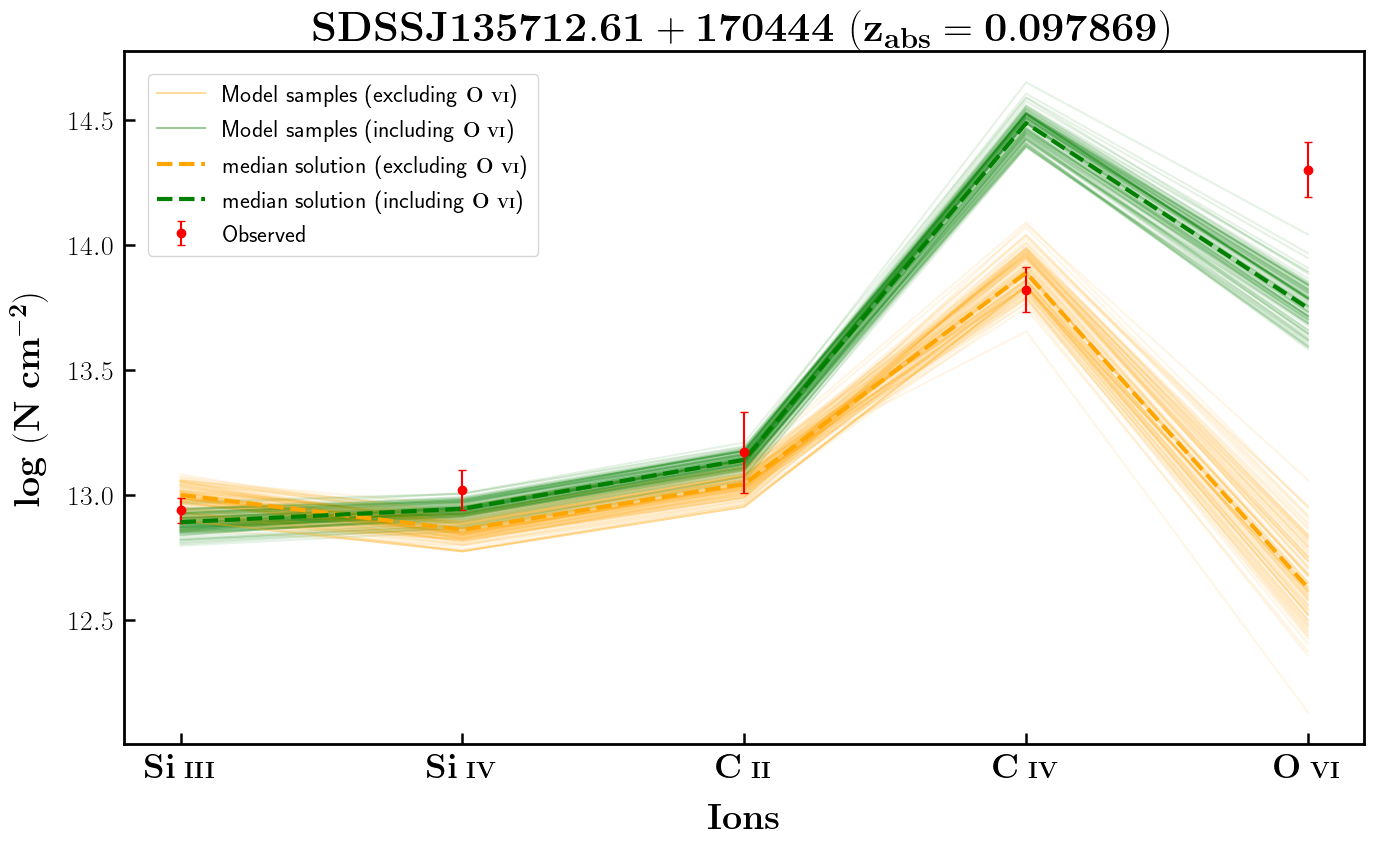
\includegraphics[width=0.85\linewidth]{Ionisation-Modelling-Plots/s135712-z=0.097869-compII.png}
    \caption{N(\ion{H}{i})=16.49}
\end{figure}

\begin{figure}[!b]
    \centering
    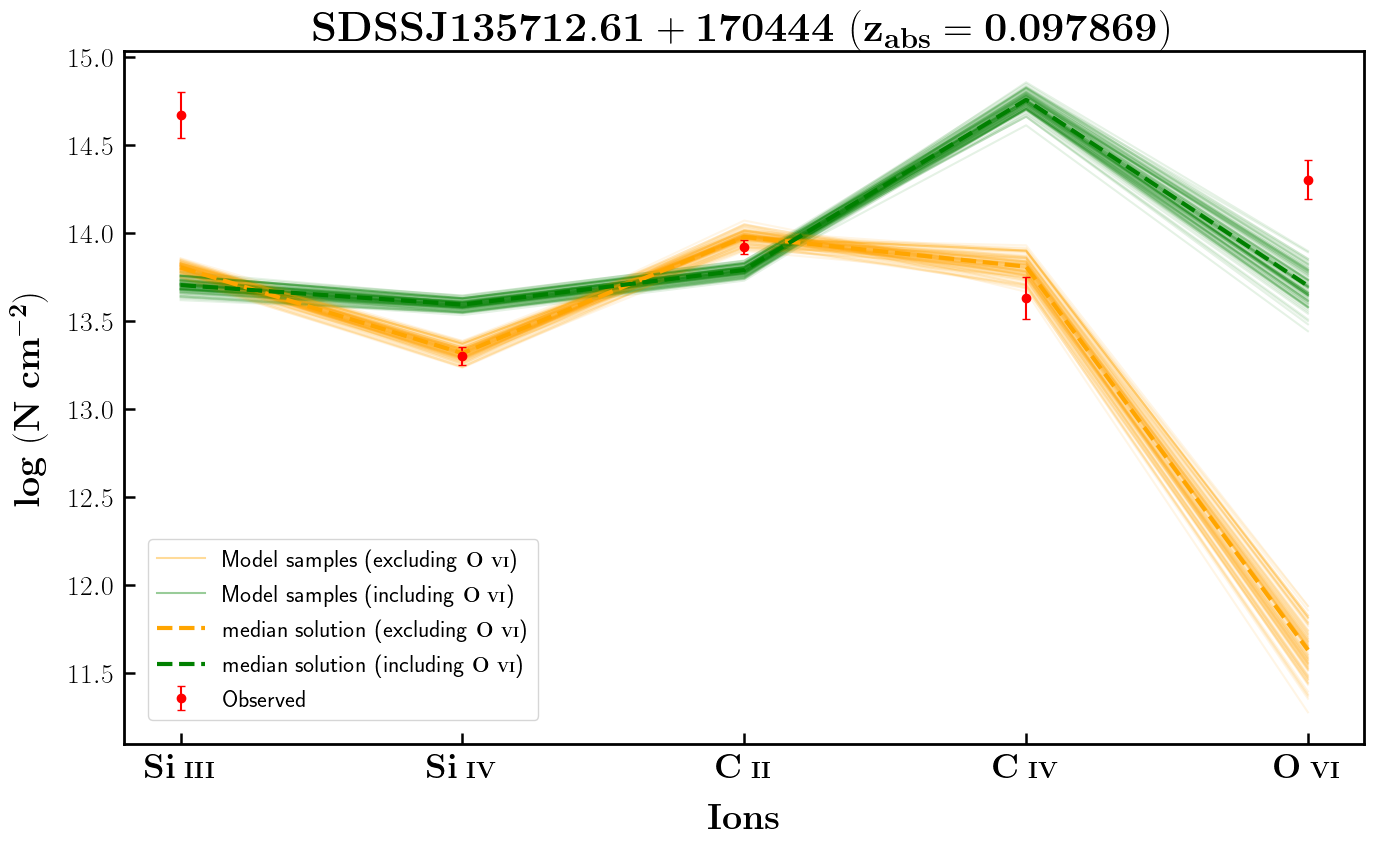
\includegraphics[width=0.85\linewidth]{Ionisation-Modelling-Plots/s135712-z=0.097869-compIII.png}
    \caption{N(\ion{H}{i})=15.01}
\end{figure}



\newpage

\begin{landscape}

\begin{figure}
    \centering
    \vspace{-20mm}
    \hspace*{-35mm}
    \captionsetup{oneside,margin={0cm,35mm}}
    \includegraphics[width=1.25\linewidth]{System-Plots/1ES1553+113_z=0.187764_sys_plot.png}
\end{figure}

\end{landscape}


\begin{center} 

\begin{tabular}{cccc} 

    \hline \hline \tabularnewline 
    \head{Ion} & \head{v (km s\textsuperscript{$\mathbf{-1}$})} & \head{b (km s\textsuperscript{$\mathbf{-1}$})} & \head{log [N cm\textsuperscript{$\mathbf{-2}$}]}
    \tabularnewline \tabularnewline \hline \tabularnewline 
 
    \ion{C}{iii}   &    -46.0 $\pm$ 1.0   &    5 $\pm$ 4    &     13.17 $\pm$ 0.46 \\
    \ion{C}{iii}   &    -6.0 $\pm$ 1.0   &    13 $\pm$ 2    &     13.21 $\pm$ 0.03 \\
    \ion{N}{v}   &    -47.0 $\pm$ 2.0   &    17 $\pm$ 0    &     13.43 $\pm$ 0.05 \\
    \ion{N}{v}   &    -5.0 $\pm$ 2.0   &    16 $\pm$ 4    &     13.33 $\pm$ 0.06 \\
    \ion{O}{vi}   &    -42.0 $\pm$ 1.0   &    3 $\pm$ 1    &     14.23 $\pm$ 0.33 \\
    \ion{O}{vi}   &    0.0 $\pm$ 1.0   &    15 $\pm$ 3    &     13.71 $\pm$ 0.03 \\
    \ion{O}{vi}   &    511.0 $\pm$ 3.0   &    28 $\pm$ 5    &     13.49 $\pm$ 0.05 \\
    \ion{H}{i}   &    -52.0 $\pm$ 3.0   &    8 $\pm$ 6    &     12.76 $\pm$ 0.15 \\
    \ion{H}{i}   &    -28.0 $\pm$ 1.0   &    51 $\pm$ 1    &     13.88 $\pm$ 0.01 \\
    \ion{H}{i}   &    425.0 $\pm$ 3.0   &    25 $\pm$ 5    &     13.02 $\pm$ 0.07 \\
    \ion{H}{i}   &    496.0 $\pm$ 2.0   &    37 $\pm$ 3    &     13.46 $\pm$ 0.03 \\

    \tabularnewline \hline \hline \tabularnewline 

\end{tabular}

\end{center}







\end{document}

